\documentclass[a4paper, 10pt]{article}
\usepackage[T1]{fontenc}
\usepackage[utf8]{inputenc}
\usepackage[slovene]{babel}
\usepackage{lmodern}
\usepackage{amsmath}
\usepackage{leftidx}
\usepackage{biblatex}
\usepackage{amssymb}
\usepackage{amsthm}
\usepackage{amsfonts}
\usepackage{graphicx}
\usepackage{wrapfig}
\usepackage{amsthm}
\usepackage{mathrsfs}
\usepackage{mathtools}
\usepackage{url}
\usepackage{subfigure}
\usepackage{multirow}
\usepackage{lipsum}
\usepackage{wrapfig}
\usepackage{tikz}
\usepackage[format=plain, font=small, labelfont=bf, textfont=it, justification=centerlast]{caption}
\usepackage{booktabs}
\usepackage{siunitx}

\newtheorem{izr}{Izrek}
\newtheorem{posl}{Posledica}[izr]

\newcounter{defcount}
\newcounter{opombe}
\newcounter{zgledcount}

\newenvironment{opomba}{\begin{flushleft}\stepcounter{opombe}\textbf{Opomba \arabic{opombe}:}}{\hfill\end{flushleft}}
\setlength{\parindent}{0mm}

\newenvironment{zgled}{\begin{flushleft}\stepcounter{zgledcount}\textbf{Zgled \arabic{zgledcount}:}}{\hfill\end{flushleft}}
\setlength{\parindent}{0mm}

\newenvironment{definicija}{\begin{flushleft}\stepcounter{defcount}\textbf{Definicija \arabic{defcount}:}}{\hfill\end{flushleft}}
\setlength{\parindent}{0mm}

\newcommand{\naslov}[1]{\textit{#1}}
\newcommand{\abs}[1]{\ensuremath{\lvert #1 \rvert}}
\newcommand{\mth}[1]{\ensuremath{\mathbb{#1}}}
\newcommand{\R}{\mth{R}}
\newcommand{\Z}{\mth{Z}}
\newcommand{\Zp}{\mth{Z}^{+}}
\newcommand{\N}{\mth{N}}
\newcommand{\No}{\mth{N}_0}
\newcommand{\C}{\mth{C}}
\newcommand{\Qu}{\mth{Q}_u}
\newcommand{\pojem}[1]{\emph{#1}}
\newcommand{\con}{\ensuremath{\mathscr{C}}}
\newcommand{\padex}[2]{\ensuremath{{#1}^{\underline{#2}}}}
\newcommand{\rastx}[2]{\ensuremath{{#1}^{\bar{#2}}}}
\newcommand{\map}[3]{\ensuremath{{#1}: {#2} \rightarrow {#3}}}
\newcommand{\pra}[3]{{#1}{\ast}({#2}) = {#3}}

\title{Fermatov poslednji izrek za n=4 in sorodni problemi}
\date{11.5.2019}
\author{Jimmy Zakeršnik}
%===============================================================================
\begin{document}
\maketitle
\thispagestyle{empty}
\newpage

Denimo, da smo veliki ljubitelji serije filmov Vojne Zvezd (Star wars) in želimo iz papirja narediti (malce prirejen) model vesoljske ladije >>Supremacy<<, kot prikazuje slika \ref{fig:mot}.

\begin{figure}[h]
\centering
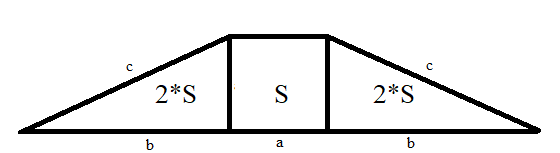
\includegraphics[scale=0.75]{Motivacijska_slika}
\caption{Skica modela, ki ga želimo sestaviti. $a$, $b$ in $c$ so pozitivna cela števila, $S$ pa površina kvadrata.}
\label{fig:mot}
\end{figure}

 Pri tem smemo papir rezati samo tako, da je dolžina vsake stranice izrezanega lika neko (pozitivno) celo število. Model želimo sestaviti iz enega kvadrata in dveh pravokotnih trikotnikov tako, da bo površina  kvadratnega lista enaka polovici površine enega trikotnega krila. Ali je to mogoče? Izkaže se, da ni.

Da odgovorimo na prejšnje vprašanje bomo dokazali s pomočjo Fermatovega poslednjega izreka, za poseben primer, ko je $n = 4$. 

\begin{izr}[Fermatov Poslednji izrek]
Naj bo $n$ celo število, ki je (strogo) večje od 2 ($n > 2$). Tedaj enačba $ x^n + y^n = z^n $ nima netrivialnih celoštevilskih rešitev $x, y, z \in \Z$
\end{izr}

Za nas bodo torej zanimive celoštevilske rešitve enačbe $x^4 + y^4 = z^4$. Preden se lotimo dokazovanja, moramo še spoznati metodo, ki bo za naš dokaz ključna: >>Metoda neskončnega spusta<<.

$ $

Z metodo neskončnega spusta najpogosteje dokazujemo, da neka dana enačba nima (oz. ima zelo malo) celoštevilskih rešitev. Najprej predpostavimo, da dana enačba ima neko celoštevilsko rešitev $a_1$, nato pokažemo, da za to rešitev obstaja še eno, na nek način manjše  celo število $a_2$, ki tudi reši enačbo. Postopek tako ponavljamo, in dobljene rešitve uredimo >>po velikosti<<, dokler ne dobimo neskončno padajočo verigo 
\[
a_1 > a_2 > a_3 > a_4 > \ldots
\]
pozitivnih celih števil, kar pa nas vodi v protislovje s Peanovim aksiomom, ki pravi, da v množici naravnih (torej pozitivnih celih) števil obstaja najmanjši element ($1$ ali $0$, odvisno od tega, koga vprašate).

Da pridobimo občutek za metodo, si jo najprej oglejmo na dveh primerih:
\newpage
\begin{izr}
Ne obstajajo takšna cela števila $x, y ~\text{in}~ z$, ki netrivialno rešijo enačbo $x^3 + py^3 + p^2z^3 = 0$, kjer je $p$ poljubno praštevilo.
\end{izr}

\begin{proof}
Naj bo $p$ poljubno praštevilo in denimo, da obstajajo takšna števila $x, y, z \in \Z$, za katera velja $(x, y, z) \neq (0,0,0)$ (torej vsaj eden izmed $x, y~\text{ali}~z$ ni enak $0$), ki rešijo dano enačbo.Potem $p$ deli $x^3$, torej $p$ deli $x$. 

$ $

Ker~$p\mid x$,~$x$ zapišemo kot $px_1$ ($x = px_1$) in ga vstavimo nazaj v enačbo. Dobimo novo enačbo $p^3x_1^3 + py^3 + p^2z^3 = 0$. Enačbo krajšamo s $p$ in jo preuredimo v $y^3 + pz^3 + p^2x_1^3 = 0$. Dobljena enačba je ekvivalentna začetni, le da smo namesto $(x, y, z)$ vstavili $(y, z, x_1)$. Zato po enakem argumentu kot prej, zapišemo $y$ kot $py_1$, da dobimo $z^3 + px_1^3 + p^2y_1^3 = 0$. Enak postopek ponovimo še za $z$ in dobimo $x_1^3 + py_1^3 + p^2z_1^3 = 0$.
Dobili smo torej trojico $(x_1, y_1, z_1)$, ki ustreza naši enačbi, in vsaj eno izmed teh števil je različno od $0$ (odvisno od tega, katero število izmed $x, y~\text{ali}~z$ je različno od $0$). 

Ker velja $0 < max(\abs{x_1}, \abs{y_1}, \abs{z_1}) = \frac{1}{p}\cdot max(\abs{x}, \abs{y}, \abs{z})$, nam je uspelo najti manjšo celoštevilsko rešitev, glede na maksimalno absolutno vrednost, kar pa je pozitivno celo število. Postopek lahko neskončnokrat ponovimo, kar pa nas privede do protislovja.
\end{proof}

\begin{izr}
Naj bo $d$ celo število, ki ni popolni kvadrat (torej ne obstaja takšno celo število $k$, da bi veljalo $d=k^2$. Potem je $\sqrt{d}$ iracionalno število.
\end{izr}

\begin{proof}
Denimo, da je $\sqrt{d}$ racionalno število. Ker $d$ ni popolni kvadrat, njegov kvadratni koren leži med dvema zaporednima celima številoma. Naj bo $l$ takšno celo število, da velja \[
l < \sqrt{d} < l+1
.\] Potem lahko $\sqrt{d}$ zapišemo kot $l + \frac{m}{n}$, kjer sta $m$ in $n$ pozitivni celi števili in $0 < \frac{m}{n} < 1$ oz. $0 < m < n$. Enačbo kvadriramo in z malo urejanja dobimo
\[
dn^2 =n^2l^2 + 2mnl + m^2
\]
oziroma
\[
n \cdot (n \cdot (d -  l^2) - 2ml) = m^2
\]
Zapis skrajšamo v $m^2 = nq$, kjer je $q = n \cdot (d -  l^2) - 2ml$. Ker sta $m^2$ in $n$ pozitivni celi števili, je tudi $q$ pozitivno celo število. Torej je $\frac{m}{n} = \frac{q}{m}$ ter 
\[
\sqrt{d} = l + \frac{m}{n} =  l + \frac{q}{m}.
\]

Poleg tega iz enakosti $\frac{m}{n} = \frac{q}{m}$ sledi še $0 < \frac{q}{m} < 1$ oz. $0 < q < m$. Ulomek $\frac{q}{m}$ ima manjši imenovalec kot $\frac{m}{n}$ in iz enakosti $\sqrt{d} - l =\frac{m}{n}$, dobimo enakost $\sqrt{d} - l =\frac{q}{m}$ z manjšim pozitivnim celoštevilskim imenovalcem. Postopek ponovimo, dokler ne dobimo neskončne padajoče verige imenovalcev in tako pridemo v protislovje.
\end{proof}

Sedaj, ko smo dobili občutek za novo metodo, se bomo lotili Fermatovega izreka. Začnimo kar z definicijo:

\begin{definicija}
Pitagorejska trojica je sestavljena iz treh celih števil $a, b, c \in \Z$, za katera velja $a^2 + b^2 = c^2$. Če so $a, b~\text{in}~c$ paroma tuja si števila, pravimo, da je trojica \textbf{primitivna}. Pitagorejsko torjico števil $a, b~\text{in}~c$ označimo z $(a, b, c)$.
\end{definicija}

Da odgovorimo na vprašanje iz uvoda, moramo ugotoviti, ali obstaja takšna Pitagorejska trojica $(a, b, c)$, da je število $\frac{a\cdot b}{2}$ (torej ploščina trikotnika) enako dvakratniku nekega popolnega kvadrata (torej ploščini kvadrata).

\begin{izr}
Naj bo $(a, b, c)$ Pitagorejska trojica in $d$ neko pozitivno celo število. Potem je ploščina trojici pripadajočega pravokotnega trikotnika enaka ploščini kvadrata s stranico dolžine $d$ natanko tedaj, ko obstaja netrivialna celoštevilska rešitev enačbe $x^4 + y^4 = z^2$
\end{izr}
\begin{proof}
Naj bo $(a, b, c)$ Pitagorejska trojica, in $2d^2 = \frac{ab}{2}$. Označimo:
\[
x = b, y = 2d, z = bc
\]

Če obstaja takšna Pitagorejska trojka, obstaja rešitev za enačbo 

\[
x^4 + y^4 = z^2
\]
Enostaven račun to takoj pokaže:
\begin{align*}
x^4 + y^4 &= z^2 \\
b^4 + (2d)^4 &= (bc)^2 \\
b^4 + 16d^4 &= b^2c^2 \\
b^4 + 16(\frac{ab}{4})^2 &= b^2c^2 \\
b^2(b^2 + a^2) &= b^2c^2 
\end{align*}
Če je $b=0$, potem se enačba očitno izide, če $b\neq 0$ pa dobimo enačbo Pitagorovega izreka.


Sedaj naj bodo $x, y~\text{in}~z$ netrivialne pozitivne celoštevilske rešitve enačbe \[x^4 + y^4 = z^2\].
Označimo:
\[
a = x^2, b = y^2, c = z, d =\frac{xy}{2}
\]
Vemo, da je $d$ celo število, saj je bodisi $x$, bodisi $y$ sodo število \\ (sicer $z^2 \equiv 2~mod~4$, kar pa ni mogoče).
Sledi, da je $(a, b, c)$ pitagorejska trojica in $2d^2 = 2 \cdot \frac{x^2y^2}{4} = \frac{x^2y^2}{2} = \frac{ab}{2}$.
\end{proof}

Kako pa je enačba $x^4 + y^4 = z^2$ povezana s Fermatovim poslednjim izrekom za $n=4$? Denimo, da je pozitivno celo število $z$ enako kvadratu nekega drugega celega števila $c$, torej $z=c^2$. Potem se $x^4 + y^4 = z^2$ spremeni v $x^4 + y^4 = c^4$. Sledi torej, da  če obstaja celoštevilska rešitev za $x^4 + y^4 = c^4$, obstaja tudi netrivialna celoštevilska rešitev za $x^4 + y^4 = z^2$.

Preden zapišemo naslednji izrek, si poglejmo še parametrizacijo primitivnih Pitagorejskih trojic, saj bomo to znanje uporabili v naslednjem dokazu.
\begin{definicija}
Primitivna rešitev, za enačbo $a^2 + b^2 = c^2$, kjer so $a, b~\text{in}~c$ pozitivna cela števila in $b$ sodo (brez škode za splošnost) se glasi:
\[
a = k^2 - l^2, b=2kl, c = k^2 + l^2,
\]
kjer je $k$ večji od $l$ ter sta si $k$ in $l$ tuji števili različnih parnosti ($gcd(k, l) = 1, k \not\equiv l~mod~2$)

\end{definicija}

\begin{izr}
\label{izr:fer}
Enačba $x^4 + y^4 = z^2$ ni rešljiva v pozitivnih celih številih.
\end{izr}

\begin{proof}
Denimo, da obstaja rešitev enačbe $x^4 + y^4 = z^2$, kjer so $x, y~\text{in}~z$ pozitivna cela števila.
Če je $p$ skupni praštevilski delitelj $x$ in $y$, potem $p^4 \mid z^2$, torej tudi $p^2 \mid z$. Iz enačbe krajšamo skupni faktor $p^4$ in dobimo podobno enačbo z manjšimi pozitivnimi vrednostmi $x_1, y_1~\text{in}~z_1$. Ta postopek ponovimo tolikokrat, da velja $gdc(x_i,y_i)=1$, $gdc(x_i,z_i)=1$ in $gdc(y_i,z_i)=1$ (zadnji dve enakosti sledita iz prve).

Ker velja $x^4 + y^4 = z^2$ in $gdc(x,y)=1$, sledi, da je vsaj eno izmed $x$ in $y$ liho število. Če bi obe bili lihi, bi pa veljalo $z^2 \equiv 2~mod~4$, kar očitno ne more biti res. Zato \textbf{brez škode za splošnost} denimo, da je $x$ liho in $y$ sodo število. Potem je $z$ liho število. Ker velja $(x^2)^2 + (y^2)^2 = z^2$, sledi da je $(x^2, y^2, z)$ primitivna Pitagorejska trojica, kjer je $y^2$ sodi člen. Trojica torej ustreza pogojem prej definirane parametrizacije.
Označimo:
\begin{align}
\label{eq:one}
x^2 = k^2 - l^2, 
\end{align}
\begin{align}
\label{eq:two}
y^2=2kl,
\end{align}
\begin{align}
\label{eq:three}
 z = k^2 + l^2,
\end{align}
kjer $k > l > 0$ in $gdc(k, l) = 1$ (velja tudi $k \not\equiv l~mod~2$, a tega tukaj ne potrebujemo). Po enačbi \ref{eq:one}~velja $x^2 + l^2 = k^2$. Ker je $gdc(k, l) = 1$ sledi, da je tudi $(x, l, k)$ primitivna Pitagorejska trojica. Ker je $x$ liho število, ponovno uporabimo parametrizacijo primitivnih Pitagorejskih trojic:
\[
x = a^2 - bl^2, l=2ab, k = a^2 + b^2,
\] 
kjer $a > b > 0$ in $gdc(a, b) = 1$.

Enačba \ref{eq:two}~sedaj izgleda takole:
\[
y^2 = 4(a^2 + b^2)ab
\]
Ker je $y$ sodo, sledi:
\[
(\frac{y}{2})^2 = (a^2 + b^2)ab
\]
Ker velja $gdc(a, b) = 1$ sledi, da so si $a^2 + b^2$, $b$ in $a$ paroma tuja števila. Ker je njihov produkt enak nekemu popolnemu kvadratu, sledi, da so tudi sami popolni kvadrati oz:
\[
a = x_1^2, b = y_1^2, a^2 + b^2 = z_1^2.
\]
Predpostaviti smemo, da so $x_1, y_1~\text{in}~z_1$ pozitivna (cela) števila. Iz $gdc(a, b) = 1$ sledi $gdc(x_1, y_1) = 1$. Če $a$ in $b$ z tretji zgornji enačbi zamenjamo z novimi oznakami, dobimo:
\[
x_1^4 + y_1^4 = z_1^2,
\]
torej smo pridobili še eno rešitev naše začetne enačbe, za katero velja $gdc(x_1, y_1) = 1$. Sedaj bomo primerjali $z$ in $z_1$. Iz prejšnjih enačb sledi naslednje:
\[
z = k^2 + l^2 = (a^2 + b^2)^2 + (2ab)^2 = z_1^4 + 4x_1^4y_1^4,
\]
torej je $z$ večji od $z_1^4$.
Sledi naslednja ocena:
\[
0 < z_1 \leq z_1^4 < z.
\]
Vsako trojico $(x, y, z)$, ki reši našo enačbo primerjamo glede na velikost zadnjega člena (torej $z$). Postopek ponavljamo, dokler ne dobimo neksončne padajoče verige, kar pa nas privede v protislovje.
\end{proof}

Enačba $x^4 + y^4 = z^2$ torej nima netrivialnih pozitivnih celoštevilskih rešitev, kar nam pove dvoje. Prvič, velja Fermatov poslednji izrek za posebni primer $n = 4$ in drugič, naš model vesoljske ladje (žal) ni mogoč. Kljub temu, gremo dokazati še par posledic prejšnjega izreka.

\begin{posl}
\label{pos:ena}
Za vsako trojico racionalnih števil $(x, y, z)$, ki rešijo enačbo $x^4 + y^4 = z^2$ velja, da je bodisi $x$, bodisi $y$ enak $0$.
\end{posl}

\begin{proof}
Predpostavimo, da tako $x$, kot $y$ nista enaka $0$. Potem je $z^2$ pozitivno število, torej tudi $z$ ni enak $0$. $x, y~\text{in}~z$ zapišemo kot ulomke:
\[
x = \frac{a}{d}, y = \frac{b}{d}~\text{in}~z=\frac{c}{d},
\]
kjer so $a, b, c~\text{in}~d$ cela števila in $d$ večji od $0$. Potem so $a, b~\text{in}~c$ različi od $0$.
\begin{align*}
x^4 + y^4 &= z^2 \\
(\frac{a}{d})^4 + (\frac{b}{d})^4 &= (\frac{c}{d})^2 \\
a^4 + b^4 = (cd)^2
\end{align*}
Brez škode za splošnost so $a, b~\text{in}~cd$ pozitivna števila (sicer lahko $a<0$ zapišemo kot $a_1 = -a$ in podobno za ostale. Enačba se glede na predznak ne spremeni.) in pridemo v protislovje z izrekom \ref{izr:fer}
\end{proof}

\begin{posl}
\label{pos:dva}
Edini racionalni rešitve enačbe $y^2 = x^4 + 1$ sta $(0, \pm1)$.
\end{posl}

\begin{proof}
Vzemimo enačbo $x^4 + z^4 = y^2$ in predpostavimo $z = 1$. Po posledici \ref{pos:ena} je $x = 0$ . Torej $y = \pm 1$.
\end{proof}

\begin{posl}
\label{pos:tri}
Edini racionalni rešitvi enačbe $2y^2 = x^4 - 1$ sta $(\pm1; 0)$.
\end{posl}

\begin{proof}
Enačbo $2y^2 = x^4 - 1$ kvadriramo in dobimo $4y^4 = x^8 - 2x^4 + 1$. Nato prištejemo $4x^2$ in dobimo $4y^4 + 4x^4 = x^8 +2x^4 + 1$. Enačbo nato delimo s $4$ in dobimo:
\[
x^4 + y^4 = (\frac{(x^4 + 1)}{2})^2.
\]
Ker $x\neq 0$ v originalni enačbi, lahko novo enačbo delimo z $x^4$ in dobimo novo enačbo:
\[
(\frac{y}{x})^4 + 1 = (\frac{(x^4 + 1)}{2x^2})^2
\]
Po posledici \ref{pos:dva} sledi, da je $\frac{y}{x} = 0$, torej je $y = 0$ in iz tega sledi, da je $x = \pm 1$
\end{proof}

\newpage

\begin{posl}
\label{pos:stiri}
Edina racionalna rešitev enačbe $y^2 = x^3 + x$ je $(0, 0)$.
\end{posl}

\begin{proof}
Najprej dano enačbo zapišemo takole kot $y^2 = x(x^2 + 1)$. Opazimo, da je $x = 0$ natanko tedaj, ko je $y = 0$. Denimo, da obstaja racionalna rešitev, ki ni $(0, 0)$ (torej $x \neq 0~\text{in}~y \neq 0$). Iz enačbe je razvidno, da more $x$ biti pozitiven. Zdaj $x$ in $y$ zapišemo kot okrajšana ulomka $x = \frac{a}{b}$ in $y = \frac{c}{d}$, kjer sta $b$ in $d$ pozitivni števili.
Naša enačba zdaj zgleda tako:
\[
(\frac{c}{d})^2 = (\frac{a}{b})^3 + \frac{a}{b}
\]
Ko odstranimo imenovalce, dobimo:
\[
b^3c^2 = d^2(a^3 + ab^2),
\]
torej $d^2 \mid b^3c^2$. Ker je $gdc(c, d) = 1$, $d^2$ deli $b^3$. Poleg tega velja $b^3 \mid d^2(a^3 + ab^2)$.
Ker je $gdc(a, b) = 1$, sta si  $b^3$ in $a^3 + ab^2$ tuji. Potem pa $b^3$ deli $d^2$. Sledi enakost $b^3 = d^2$. Zapišimo $b = t^2$ in
$d = t^3$ za neko pozitivno celo število $t$ (to lahko storimo zaradi enolične faktorizacije celih števil). Potem je $gdc(a, t) = 1$ in $gdc(c, t) = 1$.
Če zdaj v enačbo $y^2 = x^3+x$ vstavimo $x =\frac{a}{t^2}$ in $y = \frac{c}{t^3}$, po odstranitvi imenovalca dobimo $c^2 = a^3+t^4a = a(a^2+t^4)$.
Ker je $gdc(a, t) = 1$, sta si $a$ in $a^2 + t^4$ tuji pozitivni celi števili. Ker je njun produkt popolni kvadrat, morata tudi oba faktorja biti popolna kvadrata. Zapišemo:
\[
a = u^2; a^2 + t^4 = v^2.
\]
Potem je $u^4 + t^4 = v^2$. Po izreku \ref{izr:fer} je bodisi $u$, bodisi $t$ enak $0$. Ker vemo, da $t \neq 0$, sledi $u = 0$, torej je $x = 0$ in posledično je tudi $y = 0$.
\end{proof}

\begin{opomba}
Opazimo lahko, da med posledico \ref{pos:stiri} in in izrekom \ref{izr:fer} v resnici velja ekvivalenca. Denimo, da obstaja pozitivna celoštevilska rešitev za enačbo $x^4 + y^4 = z^2$.
Enačbo pomnožimo s $\frac{x^2}{y^6}$ in dobimo $(\frac{x}{y})^6 + (\frac{x}{y})^2 = (\frac{xz}{y^3})^2$. Označimo:
\[
Y =\frac{xz}{y^3}~\text{in}~X= (\frac{x}{y})^2
\]

Potem iz začetne enačbe dobimo novo:
\[
X^3 + X = Y^2.
\]
$X$ je neničelno racionalno število, torej pridemo v protislovje s posledico \ref{pos:stiri}
\end{opomba}

\newpage

\begin{thebibliography}{99}

\bibitem{bib:gardner} K. Conrad,
\naslov{Proofs by Descent},
\\\url{http://www.math.uconn.edu/~kconrad/blurbs/ugradnumthy/descent.pdf}

\bibitem{bib:pytrip} 
\naslov{Pythagorean triple},
\\\url{https://en.wikipedia.org/wiki/Pythagorean_triple}

\bibitem{bib:infdesc}
\naslov{Proof by infinite descent},
\\\url{https://en.wikipedia.org/wiki/Proof_by_infinite_descent}

\bibitem{bib:woprin}
\naslov{Well-ordering principle},
\\\url{https://en.wikipedia.org/wiki/Well-ordering_principle}

\end{thebibliography}



\end{document}